\documentclass{article}

\usepackage[T1]{fontenc}
\usepackage[utf8]{inputenc}
\usepackage[frenchb]{babel}

\usepackage{hyperref}
\usepackage{graphicx}
\usepackage{pdflscape}

\usepackage{listings}
\lstdefinestyle{customstyle}{
    basicstyle=\footnotesize,
    breakatwhitespace=false,         
    breaklines=true,                 
    captionpos=b,                    
    keepspaces=true,
	showspaces=false,   
	showstringspaces=false,	                                                                                        
    tabsize=4,
    frame=single, %lines
    moredelim=[is][\underbar]{_}{_} % underlines permitted without escape character
}
\lstset{style=customstyle}

\title{Free Basic to C compiler}
\author{Jérémy Bardon}

\begin{document}
\maketitle

\renewcommand{\contentsname}{Sommaire}
\tableofcontents	
	
\newpage
	
\section{Introduction}
Le but de ce projet\footnote{Code source disponible sur GitHub : \href{https://github.com/jbardon/fbtocc}{jbardon/fbtocc}} est de créer un compilateur capable de convertir un code écrit 
en \href{http://www.freebasic.net}{Free Basic} dans le langage C. 

\begin{figure}[h]
    \centering
    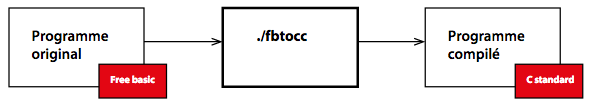
\includegraphics[scale=0.6]{resources/schema.png}
    \caption{Rôle du compilateur}
\end{figure}
	
Le programme en C
ainsi généré sera compilable avec \emph{gcc} et effectuera les mêmes opérations que 
le programme original.
	
\section{Adaptations entre les langages}
Par défaut, un programme écrit en free basic dispose comme en C d'un 
certain nombre de fonctions que l'on peut utiliser sans inclure des programmes 
externes. Cependant, ces fonctions \og{}basiques\fg{} ne sont pas équivalentes dans 
les deux langages.
\\\\
L'exemple le plus simple est la fonction qui permet d'afficher un message : en 
free basic il s'agit de la fonction \emph{print} qui est incluse 
par défaut mais en C il est nécessaire d'inclure \emph{stdio.h} pour utiliser 
la fonction \emph{printf}.
\\\\
Une autre différence de taille est la présence -- en C -- d'une routine principale 
(main) qui doit être présente dans tout programme écrit en C. Ce n'est pas le cas du 
free basic qui propose une structure plus libre du programme.

\lstset{language=c,caption=Programme C englobant}
\lstinputlisting{resources/wrap.c}

Ce sont ces différences qui amènent à devoir proposer une structure englobante d'un 
programme dans laquelle on va ensuite insérer le code free basic converti.
	
\section{Grammaire et éléments reconnus}
L'organisation des fichiers sources du compilateur permet de facilement identifier quelles sont 
les règles de grammaire ainsi que les caractères reconnus.
En effet, le fichier \emph{scanner.mll} regroupe la partie analyse syntaxique tandis que le fichier 
\emph{parser.mly} s'occupe de l'analyse syntaxique et donc de la grammaire.
\\\\
Tout les exemples utilisés lors du développement du compilateur sont disponibles dans le répertoire 
\emph{test} -- à la racine du projet -- et il contient notamment le fichier \emph{full.fba} qui peut 
donner un aperçu global de ce que le compilateur est capable de reconnaitre et de traduire.

\subsection{Variables}
Il existe de nombreux types de variables en free basic mais le compilateur reconnait seulement les types \emph{Integer}
et \emph{String} qui sont les plus utilisés. 
\\\\
Hormis la déclaration de variables et de constantes, il est possible de faire des affectations de valeurs simples
ou d'expressions plus complexes avec les symboles: $+$, $-$, $*$ et $/$.

\subsection{Fonctions}
Le compilateur gère de manière transparente l'appel à n'importe quelle fonction avec un ou plusieurs arguments
qu'ils soient donnés en dur ou via une variable.
\\\\
Cela dit, pour assurer un minimum de compatibilité avec le langage c, la fonction \emph{Print} est automatiquement
remplacée par \emph{printf}. Il n'est pas possible d'afficher plusieurs 
variables car cela aurait nécessité de construire le pattern demandé par la fonction \emph{printf}. 
L'implémentation de cette fonctionnalité est tout de même possible mais aurait demandé plus de temps.

\subsection{Commentaires}
Afin de se concentrer sur des éléments considérés plus importants -- conditions, boucles, ... --, seul les
commentaires mono-lignes sont reconnus. Cela permet tout de même d'insérer des commentaires sans donner 
la souplesse des commentaires multi-lignes.

\subsection{Conditions}
L'implémentation des structures conditionnelles est fonctionnelle dans une forme simple et n'intègre pas
l'utilisation de plusieurs clauses \emph{Else if} sous une même condition.
\\\\
Il reste tout à fait possible d'imbriquer une condition dans une clause \emph{else} d'une première condition et
même si cela rend la syntaxe plus complexe ce type d'opérations reste possible.

\lstset{language=c,caption=Raccourci de syntaxe pour les conditions, upquote=true}
\lstinputlisting{resources/condition.fba}\footnote{Commentaires en c, LaTeX refuse l'apostrophe}

Le compilateur supporte les comparateurs les plus utilisés : 	
\\\\
=, >, <, >= et <=
\\\\
Il supporte la comparaison entre 
des variables et/ou les types \emph{Integer} et \emph{String} de manière avancée puisque dans la cas d'un comparaison
entre deux chaines de caractères, celui-ci utilise la fonction générique du c \emph{strcmp} de manière automatique.
\\\\
Cela dit, il ne permet pas de comparer le résultat d'une fonction ou encore d'une expression avec une autre et il 
ne déduit pas que l'absence de comparateur est similaire à \emph{== 0}.
\subsection{Boucles}
L'ensemble des boucles -- pour et tant que -- sont implémentés et le compilateur donne un peu plus 
de souplesse lors de leur utilisation.
\\\\
En effet, il est possible en free basic de définir une boucle infinie -- qui n'a pas de condition -- et 
l'équivalent en c est de donner la condition \emph{1}. Ce type de boucles est reconnu par le 
compilateur qui converti automatiquement une boucle infinie en une boucle avec la condition \emph{1}.
\\\\
Dans certaines versions du C, il est impossible de définir une variable directement dans la clause \emph{for}.
C'est pourquoi le compilateur va se charger de créer de manière automatique la variable utilisée dans 
la construction de la boucle si elle n'a pas été déclarée auparavant.
	
\section{Reconnaissance des erreurs}
Dans sa première version -- qui est l'actuelle version --, le compilateur ne gère que un type 
d'erreur de logique -- utilisation d'une variable non déclarée -- dans le code 
en free basic en plus de détecter les défauts d'ordre syntaxiques. Il est donc capable 
de fournir le numéro de ligne et de caractère auquel il s'est arrêté si la phase
d'analyse lexicale à échoué.
\\\\
On fait donc l'hypothèse que le code en entrée est compilable et exécutable sans erreurs
ce qui permet de se concentrer d'avantage sur la reconnaissance -- et la conversion -- 
de nombreux éléments du langage.
\\\\
L'architecture interne du compilateur -- décrite section \ref{sec:Fonctionnement} -- a été pensée pour permettre
l'intégration de cette fonctionnalité. En effet, tout les éléments sont stockés sous forme
d'un arbre syntaxique et les variables sont sauvegardées dans un registre.
	
\section{Fonctionnement interne}\label{sec:Fonctionnement}
Au delà de l'analyse lexicale plutôt générique, la partie intéressante se situe au niveau
de l'analyse syntaxique. En effet, lors de cette phase on ne vérifie pas le sens que peut avoir 
une ligne de code mais 
seulement si elle est bien construite. 
\\\\
Le compilateur ne se contente pas de transformer 
chaque ligne en une autre sous forme de chaines de caractères mais il construit un 
arbre syntaxique qui permet d'identifier clairement comment s'enchainent les instructions
et quel sont leur sens (définition de variable, condition, boucle..).
\\\\
En parallèle de cet arbre, il tient à jour un registre des variables -- sous forme de 
table de hashage -- qui sont déclarés dans le programme afin de pouvoir afficher 
différemment un entier et une chaine de caractères. Ce registre retient donc le nom et le
type de chaque variable ce qui rend facilement possible la traduction d'une comparaison 
entres des entiers ou entre des chaines de caractères.
\\\\
Une fois l'arbre construit et le registre rempli, un algorithme parcours l'arbre et 
s'occupe de transformer chaque élément sous forme de chaîne de caractère correspondant
à un code C valide.

\section{Exemple concret}
\subsection{Présentation et code free basic}
Pour illustrer de manière plus explicite le fonctionnement du compilateur, prenons un 
exemple de code en free basic que l'on veux convertir en C.

\lstset{language=c,caption=Exemple en free basic}
\lstinputlisting{resources/sample.fba}

Cet exemple ne montre pas toutes les fonctionnalités que le compilateur possède ni 
l'intégralité des syntaxes reconnus mais essaye d'en montrer une partie.
\\\\
Ce programme demande un mot de passe et donne 5 essais pour y réussir. On a donc une 
variable -- qui contient l'entrée utilisateur -- puis une boucle -- dont la variable 
n'est pas déclarée -- dans laquelle un message différent est affiché selon une condition.

\subsection{Structures générées par le compilateur}
\subsubsection*{Arbre syntaxique}
\begin{landscape}
	\begin{figure}[h]
    		\centering
    		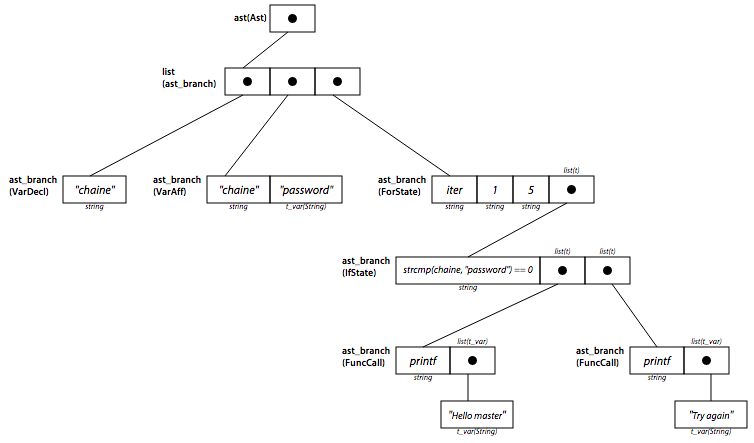
\includegraphics[scale=0.65]{resources/exemple_arbre.png}
    		\caption{Arbre syntaxique de l'exemple}
	\end{figure}
\end{landscape}

\subsubsection*{Registre des variables}
La variable utilisée dans la boucle n'apparait pas dans le registre car elle est ajoutée
au moment où l'on traduit l'instruction en C. 

\begin{figure}[h]
    \centering
    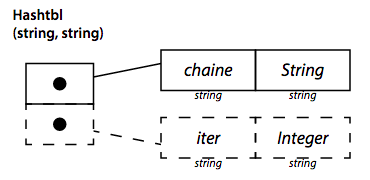
\includegraphics[scale=0.6]{resources/registre.png}
    \caption{Registre des variables}
\end{figure}

A partir du moment où cette étape est passée, 
la variable \emph{iter} est dans le registre pour permettre à la suite du programme de la
reconnaitre.

\subsection{Code généré}
Le code C généré par le compilateur se trouve dans le fichier \emph{output.c}, il est 
possible de le compiler -- et de l'exécuter -- sans problème avec un compilateur C tel que \emph{gcc}.

\lstset{language=c,caption=Code c de l'exemple}
\lstinputlisting{resources/sample.c}

On peut remarquer que le tout est indenté correctement mais il s'agit d'un traitement à la main 
pour que se soit plus lisible dans le rapport. 
\\\\
En effet, le compilateur ne gère pas 
l'indentation du code car cet aspect est moins important que la traduction du code. De plus,
lors de l'utilisation d'outils de conversion -- comme ce compilateur --, l'utilisateur ne 
s'intéresse que très rarement au code généré.

\end{document}